\documentclass[../competing_bandits.tex]{subfiles}
\begin{document}

\section{Algorithms' Performance in Isolation}\label{section:4}

We start with a pilot experiment in which we investigate each algorithm's performance "in isolation": in a stand-alone bandit problem without the competition. We focus on reputation scores (\ie sliding window averages) generated by each algorithm. 

First, we confirm that algorithms' performance is ordered as we'd expect:
    $\TS \gg \DEG \gg \DG$.
For a given algorithm and MAB instance

the reputation ordering of the algorithms is what we would expect according to the multi-armed bandit literature where, according to the mean reputation, $\TS > \DEG > DG$ for sufficiently large $t$. Second, we want to better understand what statistics of the priors we can look at in isolation in order to help us predict and understand what to expect in the competition game.

\begin{figure}
\caption{Mean Reputation Trajectories in Isolation}
\includegraphics[scale=0.35]{"figures/nih_iso_mean"}
\label{prelim_means}
\caption*{\tiny{The plots contain the average reputation over $1000$ runs for a memory size of $100$ where, for a given $t$, we record the reputation of a given algorithm on a given instance and then average this value across all the runs. The shaded area display 95\% confidence intervals.}}
\end{figure}

Figure \ref{prelim_means} shows that the mean reputation ordering is as we would expect for the Needle In Haystack prior \footnote{The mean reputation ordering that we expect also holds for the other two priors and the results for those can be found in the supplementary material.}.

\begin{figure}[H]
\caption{Reputation Distribution}
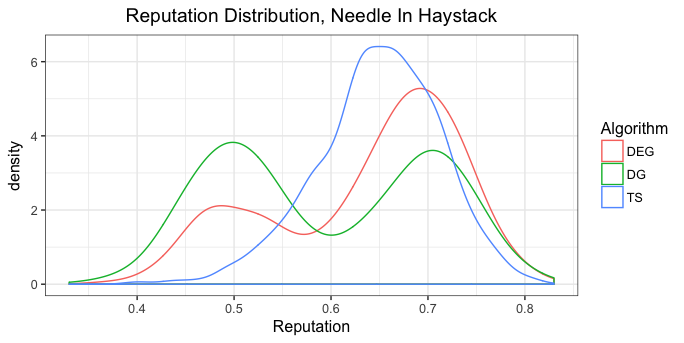
\includegraphics[scale=0.35]{figures/rep_distribution_nih}
\label{rep_dist_nih}
\caption*{\tiny{The plots contain a kernel density estimate of the reputation distribution at $t = 500$}}
\end{figure}

\begin{finding}
\textit{The mean performance of an algorithm is not a sufficient statistic for understanding the performance of an algorithm in competition. Looking at the distribution of reputation difference between algorithms we find that it tend is skewed to the right. Additionally we provide a counterexample where the mean performance does not predict the result of the competition game.}
\end{finding}


Is looking at the mean performance of between two algorithms sufficient for understanding what happens in competition? To answer this, we first look at the entire reputation distribution at $t = 500$ in Figure \ref{rep_dist_nih}. We see that the ``naive" algorithms $DG$ and $\DEG$ have a bi-modal reputation distribution whereas $\TS$ does not. The intuition for this is that, for Needle In Haystack, $DG$ either finds the best arm or not. If it does, then since it engages in no purposeful exploration it will do better than any algorithm that engages in purposeful exploration over sufficiently many rounds. However, if it does not then it will get stuck on a bad arm and lose to $\TS$ or $\DEG$. In these cases its reputation may be substantially worse but for the competition game the relative comparison between them is all that matters \footnote{This holds for our model and the decision rule of the agents, though the absolute difference may matter if, for instance, we consider the SoftMax decision rule in \cite{CompetingBandits-itcs16}}.

To better capture the comparison between two algorithms we explicitly plot the distribution of the reputation difference between $\TS$ and $DG$. This figure seems to confirm the intuition noted previously since the reputation distribution has its largest mass around the point just below 0 but it is skewed to the right even as $t$ gets large. Given the skewedness of the distribution, the mean is not a representative statistic of the entire reputation difference distribution. There are alternative statistics that we could consider such as the median or numerically calculating $\Pr(reputation(TS) - reputation(DG)) > 0$ using the estimated density, but instead we define a simple and natural statistic to help us reason about what happens under competition, the \textit{relative reputation proportion}.

\begin{figure}[H]
\caption{Reputation Difference Distribution}
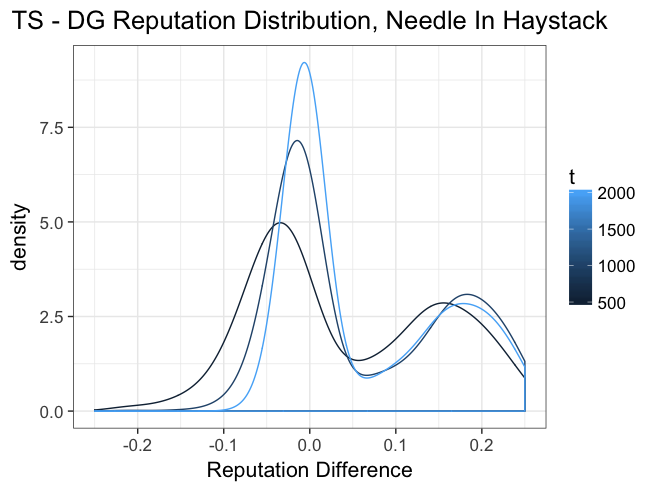
\includegraphics[scale=0.35]{figures/ts_dg_rep_diff_nih}
\label{ts_dg_rep_diff_nih}
\caption*{\tiny{The plots contain a kernel density estimate of the difference in reputation between $\TS$ and $DG$ across $t$}}
\end{figure}

\begin{definition}
\textit{Relative Reputation Proportion} - the proportion of simulations in which algorithm $A$ had at least as high of a reputation as algorithm $B$ for a fixed time $t$
\end{definition}


\begin{finding}
\textit{Purposeful exploration can lead to relative reputational costs compared to the greedy alternative and this leads to $\TS$ doing worse than $DG$ for small time horizons. We observe this under the Uniform and Heavy Tail priors. However, it is not observed under the Needle In Haystack prior}
\end{finding}

The relative reputation statistic corresponds to running the bandit algorithms in isolation on the same instance and with the same realizations for $t$ rounds and then calculating the fraction of simulations at which an agent would select a firm playing $A$ over a firm playing $B$ at time $t$ \footnote{As further motivation for this statistic, one may be interested in if there is ever a case where, for sufficiently large $t$, we observe that $\DEG >DG$ or $\TS > DG$ according to the mean reputation but $DG > \DEG$ or $DG > TS$ according to the relative reputation proportion. In the supplementary material we have results showing that, for Heavy Tail prior with $K=3$ we have that $\DEG > DG$ according to the mean reputation but $DG > \DEG$ according to the relative reputation proportion. Additionally, these results carry over to the competition game}.

\begin{figure}[ht]
\caption{Relative Reputation Plots}
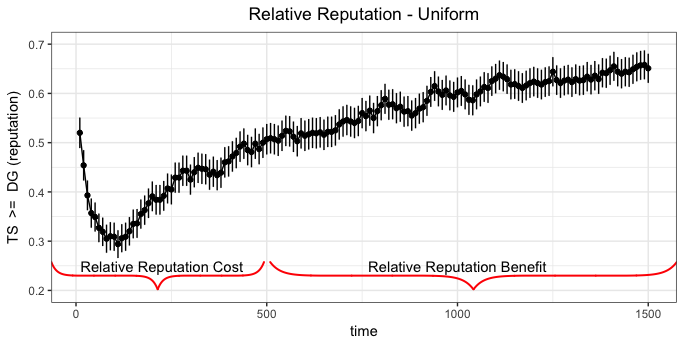
\includegraphics[scale=0.35]{figures/relative_uniform_annotated_plot}
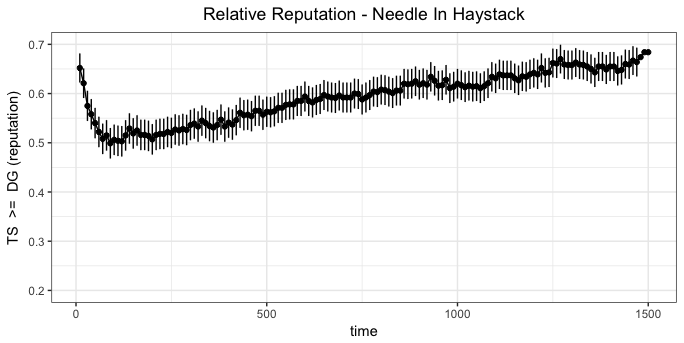
\includegraphics[scale=0.35]{figures/ts_dg_nih_10_prelim}
\caption*{\tiny{The plots contain the average reputation over $1000$ runs for a memory size of $100$ where, for a given $t$, we record the reputation of both of the algorithms on a given instance and then calculate the proportion of runs where $\TS \geq DG$. The shaded area display 95\% confidence intervals.}}
\label{relative_rep_plots}

\end{figure}



Figure \ref{relative_rep_plots} shows plots of the relative reputation proportion for $\TS$ vs $DG$ on the Uniform and Needle In Haystack prior. For the Uniform prior we see that, in the early rounds, $DG > TS$ for the majority of the simulations but that, eventually, $\TS > DG$. The intuition behind this is that, especially since the firms start with no substantive initial information, $\TS$ does purposeful exploration in the early rounds in order to acquire information. However, eventually the information acquired from purposeful exploration in the early rounds allows $\TS$ to make better decisions and achieve a higher reputation, especially when the instance is ``hard enough" so that $DG$ cannot trivially find the best arm. The early exploration leads to what we define as a \textit{relative reputation cost} and the eventual gain in reputation leads to what we define as a \textit{relative reputation benefit}.



\begin{definition}
\textit{Relative reputation cost and benefit} - the relative reputation loss an algorithm incurs from purposeful exploration compared to the greedy alternative. Here we treat it as an empirical definition based on the relative reputation proportion where the ``cost" regime is when the proportion $< 0.5$ and the ``benefit" regime is when the proportion is $> 0.5$ for the better algorithm. We call the priors where there is an early costly period followed by a later benefit period relative reputation costly priors.
\end{definition}
Is exploration always costly? Figure \ref{relative_rep_plots} also shows that for the Needle In Haystack prior, $\TS$ always does relatively better than $DG$. There are two contributing factors to this. First, $\TS$ identifies the best arm faster in the Needle In Haystack prior than the Uniform prior so that there is a shorter time horizon where $\TS$ needs to engage in purposeful exploration. Second, in the Needle In Haystack prior there are no ``bad" arms as there may be in the Uniform prior since by construction all the arms except one in Needle In Haystack are the same. Thus, when $\TS$ pulls a sub-optimal arm relative to its current information, the expected reward is the same as the greedy option that has not identified the best arm. However, with the Uniform prior, it is possible that the sub-optimal arm that is pulled has substantially lower expected reward relative to the greedy option. Thus, only the Uniform and Heavy Tail priors are relative reputation costly priors.

\end{document} 